% 1957 年全国卷第 7 题：三角形内切圆、切点 E 与高 AD。
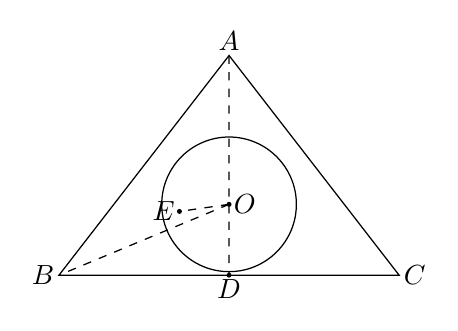
\begin{tikzpicture}[scale=0.9, line width=0.45pt,
  every node/.style={inner sep=1.5pt}]
  \coordinate (B) at (-2.4,0); \coordinate (C) at (2.4,0); \coordinate (A) at (0,3.1);
  \coordinate (D) at (0,0); \coordinate (O) at (0,1.0); \coordinate (E) at (-0.7,0.9);
  \draw (A)--(B)--(C)--cycle;
  \draw (O) circle (0.95);
  \draw[dashed] (A)--(D) (O)--(E) (O)--(B);
  \fill (O) circle (0.035) (D) circle (0.035) (E) circle (0.035);
  \node[anchor=south] at (A) {$A$}; \node[anchor=east] at (B) {$B$};
  \node[anchor=west] at (C) {$C$}; \node[anchor=north] at (D) {$D$};
  \node[anchor=west] at (O) {$O$}; \node[anchor=east] at (E) {$E$};
\end{tikzpicture}
